\documentclass[a4paper]{oblivoir}
\usepackage{amsmath,amssymb,kotex,kswrapfig,mdframed,paralist}
\usepackage{fapapersize}
\usefapapersize{210mm,297mm,10mm,*,10mm,*}

\usepackage{tabto,pifont}
\TabPositions{0.2\textwidth,0.4\textwidth,0.6\textwidth,0.8\textwidth}
\newcommand\tabb[5]{\par\noindent
\ding{172}\:{\ensuremath{#1}}
\tab\ding{173}\:\:{\ensuremath{#2}}
\tab\ding{174}\:\:{\ensuremath{#3}}
\tab\ding{175}\:\:{\ensuremath{#4}}
\tab\ding{176}\:\:{\ensuremath{#5}}}

\usepackage{graphicx}

%\pagestyle{empty}

%%% Counters
\newcounter{num}

%%% Commands
\newcommand\prob[1]
{\vs\bigskip\par\noindent\stepcounter{num} \textbf{문제 \thenum) #1}\par\noindent}

\newcommand\pb[1]{\ensuremath{\fbox{\phantom{#1}}}}

\newcommand\ba{\ensuremath{\:|\:}}

\newcommand\vs[1]{\vspace{40pt}}

\newcommand\an[1]{\bigskip\par\noindent\textbf{문제 #1)}\par\noindent}

%%% Meta Commands
\let\oldsection\section
\renewcommand\section{\clearpage\oldsection}

\let\emph\textsf

\begin{document}
\begin{center}
\LARGE종현, 추가과제 01
\end{center}
\begin{flushright}
날짜 : 2017년 \(\pb3\)월 \(\pb{10}\)일 \(\pb{월}\)요일
,\qquad
제한시간 : \pb{17년}분
,\qquad
점수 : \pb{20} / \pb{20}
\end{flushright}

%
\prob{}
10명의 학생이 있다.
\begin{enumerate}[(1)]
\item
이 10명을 일렬로 세우는 경우의 수를 구하여라.
\item
이 10명 중 3명을 뽑아 일렬로 세우는 경우의 수를 구하여라.
\item
이 10명 중 \(n\)명을 뽑아 일렬로 세우는 경우의 수가 \(90\)일 때, \(n\)의 값을 구하여라.
\end{enumerate}

%
\prob{}
여학생 \(3\)명, 남학생 \(4\)명이 일렬로 설 때,
\begin{enumerate}[(1)]
\item
여학생끼리 이웃하여 서는 경우의 수를 구하여라.
\item
여생끼리는 서로 이웃하지 않게 서는 경우의 수를 구하여라.
\end{enumerate}

%
\prob{}
special의 모든 문자를 써서 만든 순열에서
\begin{enumerate}[(1)]
\item
s가 처음에, \(p\)가 마지막에 오는 경우의 수를 구하여라.
\item
s와 p 사이에 두 개의 문자가 있는 경우의 수를 구하여라.
\item
적어도 한쪽 끝에 자음이 오는 경우의 수를 구하여라.
\end{enumerate}

%
\prob{}
다섯 개의 숫자 \(1\), \(2\), \(3\), \(4\), \(5\)를 모두 나열하여 만들 수 있는 다섯 자리 자연수가 있다.
\begin{enumerate}[(1)]
\item
이 다섯 자리 자연수는 모두 몇 개인가?
\item
32000보다 작은 자연수는 모두 몇 개인가?
\item
(2) 중에서 5의 배수는 몇 개인가?
\end{enumerate}

%
\prob{}
네 개의 숫자 \(0\), \(1\), \(2\), \(3\)이 있다.
\begin{enumerate}[(1)]
\item
이 중에서 서로 다른 세 숫자를 써서 만들 수 있는 세 자리 정수는 몇 개인가?
\item
중복을 허락할 때, 이 숫자를 써서 만들 수 있는 세 자리 정수는 몇 개인가?
\end{enumerate}

%
\prob{}
두 집합 \(X=\{1,2,3,\}\), \(Y=\{4,5,6,7\}\)이 있다.
\begin{enumerate}[(1)]
\item
집합 \(X\)에서 집합 \(Y\)로의 함수의 개수를 구하여라.
\item
집합 \(X\)에서 집합 \(Y\)로의 일대일함수의 개수를 구하여라.
\end{enumerate}

%
\prob{}
success의 7개의 문자를 모두 일렬로 나열할 때, 다음 물음에 답하여라.
\begin{enumerate}[(1)]
\item
나열하는 방법의 수를 구하여라.
\item
양 끝에 s가 오도록 나열하는 방법의 수를 구하여라.
\item
세 개의 s가 모두 이웃하도록 나열하는 방법의 수를 구하여라.
\end{enumerate}

%
\prob{}
\begin{minipage}{0.45\textwidth}
다음 그림과 같은 길을 따라 \(A\)지점에서 \(B\)지점까지 가려고 한다.
\begin{enumerate}[(1)]
\item
최단거리의 길은 몇 가지 있는가?
\item
\(A\)에서 \(P\)를 거쳐 \(B\)로 가는 최단거리의 길은 몇 가지 있는가?
\item
대각선인 길 \(l\)은 지날 수 없다고 할 때, 최단 거리의 길은 몇 가지 있는가?
\end{enumerate}
\end{minipage}
\begin{minipage}{0.45\textwidth}
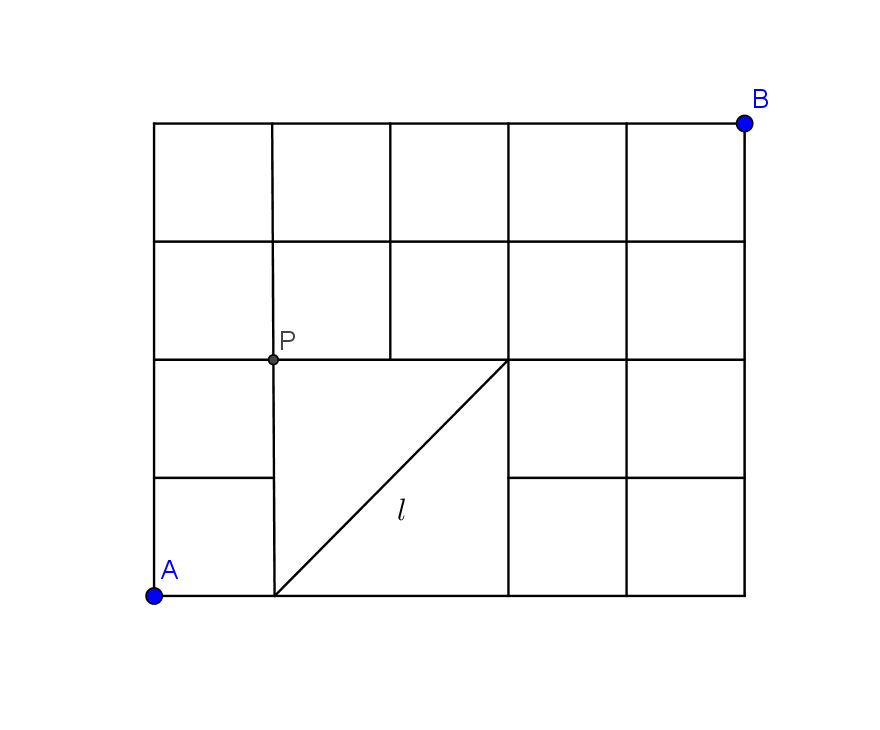
\includegraphics[width=0.8\textwidth]{ways}
\end{minipage}

%
\prob{}
네 쌍의 부부가 원탁에 둘러앉을 때, 각 쌍의 부부끼리 이웃하여 앉는 방법의 수를 구하여라.
\end{document}